\documentclass{extbook}[14pt]
\usepackage{multicol, enumerate, enumitem, hyperref, color, soul, setspace, parskip, fancyhdr, amssymb, amsthm, amsmath, latexsym, units, mathtools}
\everymath{\displaystyle}
\usepackage[headsep=0.5cm,headheight=0cm, left=1 in,right= 1 in,top= 1 in,bottom= 1 in]{geometry}
\usepackage{dashrule}  % Package to use the command below to create lines between items
\newcommand{\litem}[1]{\item #1

\rule{\textwidth}{0.4pt}}
\pagestyle{fancy}
\lhead{}
\chead{Answer Key for Makeup Progress Quiz 2 Version A}
\rhead{}
\lfoot{2790-1423}
\cfoot{}
\rfoot{Summer C 2021}
\begin{document}
\textbf{This key should allow you to understand why you choose the option you did (beyond just getting a question right or wrong). \href{https://xronos.clas.ufl.edu/mac1105spring2020/courseDescriptionAndMisc/Exams/LearningFromResults}{More instructions on how to use this key can be found here}.}

\textbf{If you have a suggestion to make the keys better, \href{https://forms.gle/CZkbZmPbC9XALEE88}{please fill out the short survey here}.}

\textit{Note: This key is auto-generated and may contain issues and/or errors. The keys are reviewed after each exam to ensure grading is done accurately. If there are issues (like duplicate options), they are noted in the offline gradebook. The keys are a work-in-progress to give students as many resources to improve as possible.}

\rule{\textwidth}{0.4pt}

\begin{enumerate}\litem{
Which of the following equations \textit{could} be of the graph presented below?

\begin{center}
    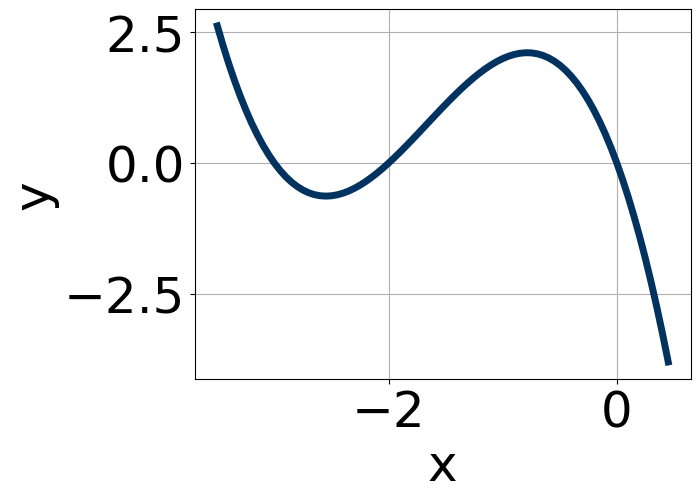
\includegraphics[width=0.5\textwidth]{../Figures/polyGraphToFunctionA.png}
\end{center}


The solution is \( -19x^{11} (x + 2)^{9} (x + 3)^{9} \), which is option A.\begin{enumerate}[label=\Alph*.]
\item \( -19x^{11} (x + 2)^{9} (x + 3)^{9} \)

* This is the correct option.
\item \( 8x^{7} (x + 2)^{11} (x + 3)^{9} \)

This corresponds to the leading coefficient being the opposite value than it should be.
\item \( -2x^{9} (x + 2)^{10} (x + 3)^{8} \)

The factors $-2$ and $-3$ have have been odd power.
\item \( -19x^{5} (x + 2)^{8} (x + 3)^{9} \)

The factor $-2$ should have been an odd power.
\item \( 15x^{9} (x + 2)^{6} (x + 3)^{7} \)

The factor $(x + 2)$ should have an odd power and the leading coefficient should be the opposite sign.
\end{enumerate}

\textbf{General Comment:} General Comments: Draw the x-axis to determine which zeros are touching (and so have even multiplicity) or cross (and have odd multiplicity).
}
\litem{
Construct the lowest-degree polynomial given the zeros below. Then, choose the intervals that contain the coefficients of the polynomial in the form $ax^3+bx^2+cx+d$.
\[ \frac{-3}{2}, -7, \text{ and } \frac{7}{2} \]The solution is \( 4x^{3} +20 x^{2} -77 x -147 \), which is option A.\begin{enumerate}[label=\Alph*.]
\item \( a \in [1, 7], b \in [20, 23], c \in [-77, -71], \text{ and } d \in [-149, -143] \)

* $4x^{3} +20 x^{2} -77 x -147$, which is the correct option.
\item \( a \in [1, 7], b \in [-20, -13], c \in [-77, -71], \text{ and } d \in [147, 150] \)

$4x^{3} -20 x^{2} -77 x + 147$, which corresponds to multiplying out $(2x -3)(x -7)(2x + 7)$.
\item \( a \in [1, 7], b \in [6, 15], c \in [-120, -118], \text{ and } d \in [147, 150] \)

$4x^{3} +8 x^{2} -119 x + 147$, which corresponds to multiplying out $(2x -3)(x + 7)(2x -7)$.
\item \( a \in [1, 7], b \in [20, 23], c \in [-77, -71], \text{ and } d \in [147, 150] \)

$4x^{3} +20 x^{2} -77 x + 147$, which corresponds to multiplying everything correctly except the constant term.
\item \( a \in [1, 7], b \in [-52, -47], c \in [158, 164], \text{ and } d \in [-149, -143] \)

$4x^{3} -48 x^{2} +161 x -147$, which corresponds to multiplying out $(2x -3)(x -7)(2x -7)$.
\end{enumerate}

\textbf{General Comment:} To construct the lowest-degree polynomial, you want to multiply out $(2x + 3)(x + 7)(2x -7)$
}
\litem{
Describe the zero behavior of the zero $x = -7$ of the polynomial below.
\[ f(x) = -2(x - 4)^{8}(x + 4)^{5}(x + 7)^{10}(x - 7)^{9} \]The solution is the graph below, which is option B.
    \begin{center}
        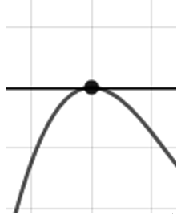
\includegraphics[width=0.3\textwidth]{../Figures/polyZeroBehaviorCopyBA.png}
    \end{center}\begin{enumerate}[label=\Alph*.]
\begin{multicols}{2}
\item 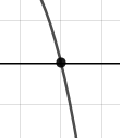
\includegraphics[width = 0.3\textwidth]{../Figures/polyZeroBehaviorCopyAA.png}
\item 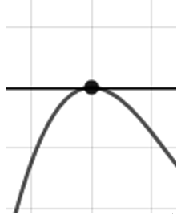
\includegraphics[width = 0.3\textwidth]{../Figures/polyZeroBehaviorCopyBA.png}
\item 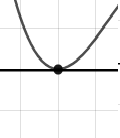
\includegraphics[width = 0.3\textwidth]{../Figures/polyZeroBehaviorCopyCA.png}
\item 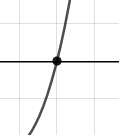
\includegraphics[width = 0.3\textwidth]{../Figures/polyZeroBehaviorCopyDA.png}
\end{multicols}\item None of the above.\end{enumerate}
\textbf{General Comment:} You will need to sketch the entire graph, then zoom in on the zero the question asks about.
}
\litem{
Describe the end behavior of the polynomial below.
\[ f(x) = 7(x - 7)^{2}(x + 7)^{3}(x - 8)^{5}(x + 8)^{5} \]The solution is the graph below, which is option D.
    \begin{center}
        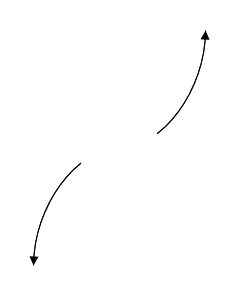
\includegraphics[width=0.3\textwidth]{../Figures/polyEndBehaviorCopyDA.png}
    \end{center}\begin{enumerate}[label=\Alph*.]
\begin{multicols}{2}
\item 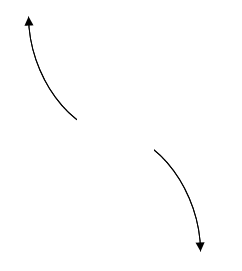
\includegraphics[width = 0.3\textwidth]{../Figures/polyEndBehaviorCopyAA.png}
\item 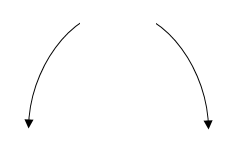
\includegraphics[width = 0.3\textwidth]{../Figures/polyEndBehaviorCopyBA.png}
\item 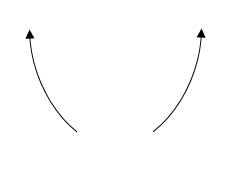
\includegraphics[width = 0.3\textwidth]{../Figures/polyEndBehaviorCopyCA.png}
\item 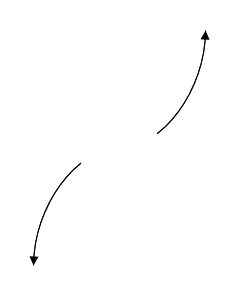
\includegraphics[width = 0.3\textwidth]{../Figures/polyEndBehaviorCopyDA.png}
\end{multicols}\item None of the above.\end{enumerate}
\textbf{General Comment:} Remember that end behavior is determined by the leading coefficient AND whether the \textbf{sum} of the multiplicities is positive or negative.
}
\litem{
Describe the end behavior of the polynomial below.
\[ f(x) = 2(x - 2)^{4}(x + 2)^{7}(x - 4)^{2}(x + 4)^{2} \]The solution is the graph below, which is option D.
    \begin{center}
        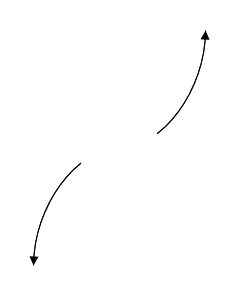
\includegraphics[width=0.3\textwidth]{../Figures/polyEndBehaviorDA.png}
    \end{center}\begin{enumerate}[label=\Alph*.]
\begin{multicols}{2}
\item 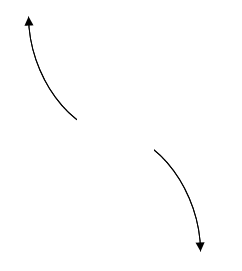
\includegraphics[width = 0.3\textwidth]{../Figures/polyEndBehaviorAA.png}
\item 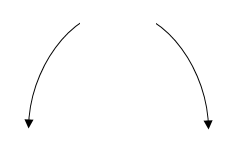
\includegraphics[width = 0.3\textwidth]{../Figures/polyEndBehaviorBA.png}
\item 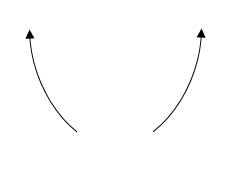
\includegraphics[width = 0.3\textwidth]{../Figures/polyEndBehaviorCA.png}
\item 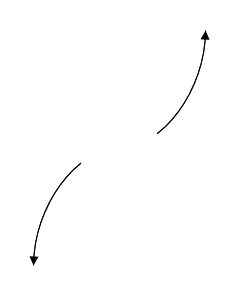
\includegraphics[width = 0.3\textwidth]{../Figures/polyEndBehaviorDA.png}
\end{multicols}\item None of the above.\end{enumerate}
\textbf{General Comment:} Remember that end behavior is determined by the leading coefficient AND whether the \textbf{sum} of the multiplicities is positive or negative.
}
\litem{
Construct the lowest-degree polynomial given the zeros below. Then, choose the intervals that contain the coefficients of the polynomial in the form $x^3+bx^2+cx+d$.
\[ -4 + 4 i \text{ and } 4 \]The solution is \( x^{3} +4 x^{2} -128 \), which is option D.\begin{enumerate}[label=\Alph*.]
\item \( b \in [0.9, 3.2], c \in [-3, 3], \text{ and } d \in [-18, -14] \)

$x^{3} + x^{2} -16$, which corresponds to multiplying out $(x + 4)(x -4)$.
\item \( b \in [0.9, 3.2], c \in [-10, -7], \text{ and } d \in [13, 21] \)

$x^{3} + x^{2} -8 x + 16$, which corresponds to multiplying out $(x -4)(x -4)$.
\item \( b \in [-7.8, -3.9], c \in [-3, 3], \text{ and } d \in [121, 134] \)

$x^{3} -4 x^{2} + 128$, which corresponds to multiplying out $(x-(-4 + 4 i))(x-(-4 - 4 i))(x + 4)$.
\item \( b \in [3.1, 5.5], c \in [-3, 3], \text{ and } d \in [-130, -123] \)

* $x^{3} +4 x^{2} -128$, which is the correct option.
\item \( \text{None of the above.} \)

This corresponds to making an unanticipated error or not understanding how to use nonreal complex numbers to create the lowest-degree polynomial. If you chose this and are not sure what you did wrong, please contact the coordinator for help.
\end{enumerate}

\textbf{General Comment:} Remember that the conjugate of $a+bi$ is $a-bi$. Since these zeros always come in pairs, we need to multiply out $(x-(-4 + 4 i))(x-(-4 - 4 i))(x-(4))$.
}
\litem{
Construct the lowest-degree polynomial given the zeros below. Then, choose the intervals that contain the coefficients of the polynomial in the form $ax^3+bx^2+cx+d$.
\[ -3, \frac{-5}{2}, \text{ and } \frac{-1}{5} \]The solution is \( 10x^{3} +57 x^{2} +86 x + 15 \), which is option A.\begin{enumerate}[label=\Alph*.]
\item \( a \in [10, 15], b \in [51, 61], c \in [80, 87], \text{ and } d \in [11, 19] \)

* $10x^{3} +57 x^{2} +86 x + 15$, which is the correct option.
\item \( a \in [10, 15], b \in [-53, -46], c \in [53, 71], \text{ and } d \in [11, 19] \)

$10x^{3} -53 x^{2} +64 x + 15$, which corresponds to multiplying out $(x -3)(2x -5)(5x + 1)$.
\item \( a \in [10, 15], b \in [-57, -54], c \in [80, 87], \text{ and } d \in [-17, -7] \)

$10x^{3} -57 x^{2} +86 x -15$, which corresponds to multiplying out $(x -3)(2x -5)(5x -1)$.
\item \( a \in [10, 15], b \in [-3, 6], c \in [-81, -75], \text{ and } d \in [-17, -7] \)

$10x^{3} -3 x^{2} -76 x -15$, which corresponds to multiplying out $(x -3)(2x + 5)(5x + 1)$.
\item \( a \in [10, 15], b \in [51, 61], c \in [80, 87], \text{ and } d \in [-17, -7] \)

$10x^{3} +57 x^{2} +86 x -15$, which corresponds to multiplying everything correctly except the constant term.
\end{enumerate}

\textbf{General Comment:} To construct the lowest-degree polynomial, you want to multiply out $(x + 3)(2x + 5)(5x + 1)$
}
\litem{
Which of the following equations \textit{could} be of the graph presented below?

\begin{center}
    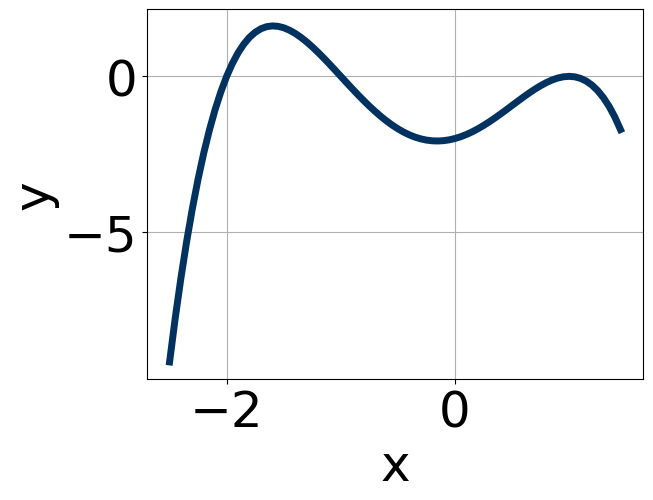
\includegraphics[width=0.5\textwidth]{../Figures/polyGraphToFunctionCopyA.png}
\end{center}


The solution is \( -15(x - 1)^{8} (x + 1)^{11} (x + 2)^{7} \), which is option A.\begin{enumerate}[label=\Alph*.]
\item \( -15(x - 1)^{8} (x + 1)^{11} (x + 2)^{7} \)

* This is the correct option.
\item \( -11(x - 1)^{8} (x + 1)^{6} (x + 2)^{9} \)

The factor $(x + 1)$ should have an odd power.
\item \( 16(x - 1)^{8} (x + 1)^{9} (x + 2)^{11} \)

This corresponds to the leading coefficient being the opposite value than it should be.
\item \( -14(x - 1)^{7} (x + 1)^{8} (x + 2)^{9} \)

The factor $1$ should have an even power and the factor $-1$ should have an odd power.
\item \( 11(x - 1)^{4} (x + 1)^{11} (x + 2)^{4} \)

The factor $(x + 2)$ should have an odd power and the leading coefficient should be the opposite sign.
\end{enumerate}

\textbf{General Comment:} General Comments: Draw the x-axis to determine which zeros are touching (and so have even multiplicity) or cross (and have odd multiplicity).
}
\litem{
Construct the lowest-degree polynomial given the zeros below. Then, choose the intervals that contain the coefficients of the polynomial in the form $x^3+bx^2+cx+d$.
\[ -3 - 4 i \text{ and } -2 \]The solution is \( x^{3} +8 x^{2} +37 x + 50 \), which is option C.\begin{enumerate}[label=\Alph*.]
\item \( b \in [-1, 5], c \in [1.8, 5.3], \text{ and } d \in [5.8, 6.4] \)

$x^{3} + x^{2} +5 x + 6$, which corresponds to multiplying out $(x + 3)(x + 2)$.
\item \( b \in [-1, 5], c \in [5.2, 8.8], \text{ and } d \in [7.7, 10.7] \)

$x^{3} + x^{2} +6 x + 8$, which corresponds to multiplying out $(x + 4)(x + 2)$.
\item \( b \in [4, 9], c \in [35.8, 38.9], \text{ and } d \in [46.8, 52.1] \)

* $x^{3} +8 x^{2} +37 x + 50$, which is the correct option.
\item \( b \in [-9, -3], c \in [35.8, 38.9], \text{ and } d \in [-50.4, -49] \)

$x^{3} -8 x^{2} +37 x -50$, which corresponds to multiplying out $(x-(-3 - 4 i))(x-(-3 + 4 i))(x -2)$.
\item \( \text{None of the above.} \)

This corresponds to making an unanticipated error or not understanding how to use nonreal complex numbers to create the lowest-degree polynomial. If you chose this and are not sure what you did wrong, please contact the coordinator for help.
\end{enumerate}

\textbf{General Comment:} Remember that the conjugate of $a+bi$ is $a-bi$. Since these zeros always come in pairs, we need to multiply out $(x-(-3 - 4 i))(x-(-3 + 4 i))(x-(-2))$.
}
\litem{
Describe the zero behavior of the zero $x = -8$ of the polynomial below.
\[ f(x) = -2(x - 8)^{8}(x + 8)^{11}(x + 9)^{9}(x - 9)^{13} \]The solution is the graph below, which is option D.
    \begin{center}
        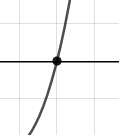
\includegraphics[width=0.3\textwidth]{../Figures/polyZeroBehaviorDA.png}
    \end{center}\begin{enumerate}[label=\Alph*.]
\begin{multicols}{2}
\item 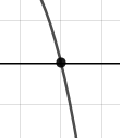
\includegraphics[width = 0.3\textwidth]{../Figures/polyZeroBehaviorAA.png}
\item 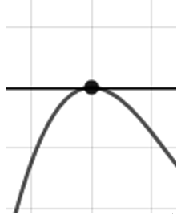
\includegraphics[width = 0.3\textwidth]{../Figures/polyZeroBehaviorBA.png}
\item 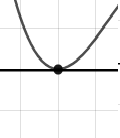
\includegraphics[width = 0.3\textwidth]{../Figures/polyZeroBehaviorCA.png}
\item 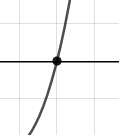
\includegraphics[width = 0.3\textwidth]{../Figures/polyZeroBehaviorDA.png}
\end{multicols}\item None of the above.\end{enumerate}
\textbf{General Comment:} You will need to sketch the entire graph, then zoom in on the zero the question asks about.
}
\end{enumerate}

\end{document}